
%\begin{wrapfigure}{l}{0.15\textwidth}                    
 \pstart  Sin vero tensio\protect\index{Sachverzeichnis}{tensio} sola aeri violenta est, compressio\protect\index{Sachverzeichnis}{compressio} non nisi per accidens, quatenus sequitur tensionem\protect\index{Sachverzeichnis}{tensio}, tunc tensionis\protect\index{Sachverzeichnis}{tensio} \edtext{augmentum idem proportione quod}{\lemma{tensionis}\Afootnote{ \textit{ (1) }\ gradus idem qu \textit{ (2) }\ augmentum idem   \textbar\ proportione \textit{ erg.}\ \textbar\  quod \textit{ L}}} superiore casu, esse debet. Fuerat scilicet spatium sequens prioris duplum, seu tensio\protect\index{Sachverzeichnis}{tensio} ante lapsum dimidia spatii post lapsum ab eodem aere occupati, ergo et nunc aer \textit{A-cc} qui occupati pedes duos \edtext{ante lapsum}{\lemma{ante}\Afootnote{lapsum \textit{ erg.} \textit{ L}}} debet occupare pedes quatuor post lapsum, et proinde Mercurius\protect\index{Sachverzeichnis}{mercurius} labetur ex \textit{cc-dd} in \textit{cccc-dddd}.
 \pend
%Zeitz auskommentiert               \begin{center}
%                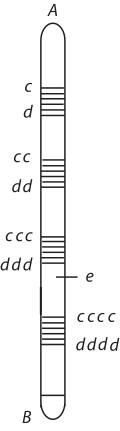
\includegraphics[width=0.2\textwidth]{images/37_3_110v}\\\textit{[Fig. 12]}
%                        %\caption{Bildbeschreibung}
%                     %   \end{wrapfigure}
%                        \end{center}
 \pstart  Sin et Tensio\protect\index{Sachverzeichnis}{tensio} et compressio\protect\index{Sachverzeichnis}{compressio} aeri violenta est, conabitur utraque retinere gradum mutationis priorem. Ergo cum ante lapsum $\rule[-4mm]{0mm}{10mm}\displaystyle\frac{11}{4}$
%
% \newline  \begin{edarrayc}
%&\cancel{4}&3&&\\
%\cancel{1}&\cancel{1}&\cancel{9}&f&\displaystyle7\frac{3}{16}\\
%&\cancel{1}&\cancel{6}&&
%\end{edarrayc} 
                    \edtext{ped.}{\lemma{Ergo}\Afootnote{ \textit{ (1) }\ ex  2 ped \textit{ (2) }\ cum ante lapsum $\displaystyle\protect\frac{11}{4}$ ped. \textit{ L}}} occupentur ab aere superiore, et $\rule[-4mm]{0mm}{10mm}\displaystyle\frac{9}{4}$ %\newline
  %  \begin{edarrayc}\displaystyle
    %\frac{88}{16}\\
   % \edatleft[hallo]{\{}{0\baselineskip}\rule[0mm]{0mm}{5mm}\\
    %\frac{27}{16}
    %\end{edarrayc}
 %
    %                
                    % \begin{wrapfigure}{l}{0.4\textwidth}                    
                %\includegraphics[width=0.4\textwidth]{../images/Propositio+experimentorum+novorum/LH037%2C03_111r/files/100200.png}
                        %\caption{Bildbeschreibung}
                        %\end{wrapfigure}
                        %@ @ @ Dies ist eine Abstandszeile - fuer den Fall, dass mehrere figures hintereinander kommen, ohne dass dazwischen laengerer Text steht. Dies kann zu einer Fahlermeldung fuehren. @ @ @ \\
                     ab aere inferiore; post lapsum ($\displaystyle\frac{88}{16}$)% \begin{wrapfigure}{l}{0.4\textwidth}                    
                %\includegraphics[width=0.4\textwidth]{../images/Propositio+experimentorum+novorum/LH037%2C03_111r/files/100204.png}
                        %\caption{Bildbeschreibung}
                        %\end{wrapfigure}
                        %@ @ @ Dies ist eine Abstandszeile - fuer den Fall, dass mehrere figures hintereinander kommen, ohne dass dazwischen laengerer Text steht. Dies kann zu einer Fahlermeldung fuehren. @ @ @ \\
                    %  \begin{tabular}{c}115-88-5\\23-88-1\end{tabular}
                    %\begin{wrapfigure}{l}{0.4\textwidth}                    
                %\includegraphics[width=0.4\textwidth]{../images/Propositio+experimentorum+novorum/LH037%2C03_111r/files/100206.png}
                        %\caption{Bildbeschreibung}
                        %\end{wrapfigure}
                        %@ @ @ Dies ist eine Abstandszeile - fuer den Fall, dass mehrere figures hintereinander kommen, ohne dass dazwischen laengerer Text steht. Dies kann zu einer Fahlermeldung fuehren. @ @ @ \\
                    $\rule[-4mm]{0mm}{10mm}\displaystyle\frac{22}{4}$ ab aere superiore et $\rule[-4mm]{0mm}{10mm}\displaystyle\frac{27}{16}$
                     %\newline
                     %\begin{edarrayl}
                     %1&&&\\
                     %\cancel{2}&9&&\\
                     %\cancel{8}&\cancel{8}&f&3\displaystyle\frac{19}{23}\\
                     %\cancel{2}&\cancel{3}&&
                     %\end{edarrayl}
                     % \begin{wrapfigure}{l}{0.4\textwidth}                    
                %
\includegraphics[width=0.4\textwidth]{../images/Propositio+experimentorum+novorum/LH037%2C03_111r/files/100208.png}
                        %\caption{Bildbeschreibung}
                        %\end{wrapfigure}
                        %@ @ @ Dies ist eine Abstandszeile - fuer den Fall, dass mehrere figures hintereinander kommen, ohne dass dazwischen laengerer Text steht. Dies kann zu einer Fahlermeldung fuehren. @ @ @ \\
                     ab inferiore tenebuntur. Erunt in summa\newline \begin{edarrayr}
\cancel{4}3&&\\
\cancel{1}\cancel{1}\cancel{5}&f&\displaystyle7\frac{3}{16}\\
\cancel{1}\cancel{6}&&
\end{edarrayr} 
% \begin{wrapfigure}{l}{0.4\textwidth}                    
                %\includegraphics[width=0.4\textwidth]{../images/Propositio+experimentorum+novorum/LH037%2C03_111r/files/100212.png}
                        %\caption{Bildbeschreibung}
                        %\end{wrapfigure}
                        %@ @ @ Dies ist eine Abstandszeile - fuer den Fall, dass mehrere figures hintereinander kommen, ohne dass dazwischen laengerer Text steht. Dies kann zu einer Fahlermeldung fuehren. @ @ @ \\
                     pedum, cum debeant esse \edtext{[5]}{\lemma{}\Afootnote{5 \textit{ erg.} \textit{ Hrsg. }\ }}, supputetur ergo in regula trium $\rule[-4mm]{0mm}{10mm}\displaystyle\frac{115}{16}$ dant $\displaystyle\left\{\begin{array}{c}\displaystyle\frac{88}{16}\\\hspace{2pt}\\\displaystyle\frac{27}{16}\end{array}\right.$\\
              %       quid dant 5 seu $%\rule[-4mm]{0mm}{10mm}
           %          \displaystyle\frac{20}{16}$   %\\\vspace{-1cm}\\
                     \begin{edarrayr}
                &     &&1\hspace{5.5pt}&&\\
              \text{quid dant 5 seu } %\rule[-4mm]{0mm}{10mm}
                     \displaystyle\frac{20}{16}    & 115-88-5&&\cancel{2}9&&\\
               %     115&-&88&-&5&&\cancel{2}9&&\\
                      & 23-88-1&f&\cancel{8}\cancel{8}&f&3\displaystyle\frac{19}{23}.
                     \edtext{}{\lemma{\ $3\displaystyle\frac{19}{23}$.}\linenum{|4|||6|}\Afootnote{ \textit{ (1) }\ Nam si sola compressio\protect\index{Sachverzeichnis}{compressio|textit} aeri violenta est non etiam tensio\protect\index{Sachverzeichnis}{tensio|textit}, \textit{ (2) }\ Esto \textit{ L}}}\\
                    & &&\cancel{2}\cancel{3}&&
                     \end{edarrayr}              
                    
% Zeitz auskommentiert                     \startlock  
%                                          % \begin{wrapfigure}{l}{0.4\textwidth}                 
%                     \begin{center}   
%                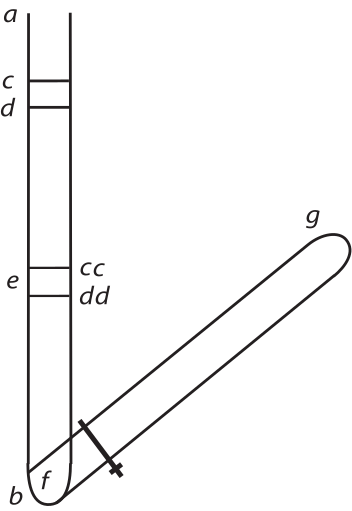
\includegraphics[width=0.3\textwidth]{images/37_3_111r}\\\textit{[Fig. 13]}\rule[-5mm]{0cm}{5mm}
%                        %\caption{Bildbeschreibung}
%                        \end{center}
%        \endlock       
        
        \setline{6}    Esto Tubus \textit{ab} % \begin{wrapfigure}{l}{0.4\textwidth}                    
                %\includegraphics[width=0.4\textwidth]{../images/Propositio+experimentorum+novorum/LH037%2C03_111r/files/100251.png}
                        %\caption{Bildbeschreibung}
                        %\end{wrapfigure}
                        %@ @ @ Dies ist eine Abstandszeile - fuer den Fall, dass mehrere figures hintereinander kommen, ohne dass dazwischen laengerer Text steht. Dies kann zu einer Fahlermeldung fuehren. @ @ @ \\
           \edtext{supra apertus}{\lemma{}\linenum{|6|||6|}\Afootnote{supra apertus \textit{ erg.} \textit{ L}}} in quo Merc.\protect\index{Sachverzeichnis}{mercurius} \textit{cd} descendens premit aerem \textit{db} comprimitque ad certum usque gradum v. g. aerem spatii \textit{db} in \edtext{spatium dimidium \textit{eb} in tubum}{\lemma{in}\linenum{|7|||8|}\Afootnote{ \textit{ (1) }\ aerem spatii dimidii \textit{eb} connectatur Tubo \textit{ (2) }\ spatium dimidium \textit{eb} in tubum \textit{ L}}} \textit{ab} inseratur?  Tubus \textit{bg} tantae \edtext{capacitatis}{\lemma{tantae}\linenum{|8|||8|}\Afootnote{ \textit{ (1) }\ longitudinis \textit{ (2) }\ capacitatis \textit{ L}}} quanta \textit{db} Epistomioque\protect\index{Sachverzeichnis}{epistomium} aperto detur communicatio, dividetur compressio\protect\index{Sachverzeichnis}{compressio} per totum \textit{ebg}. Nam aer in \textit{d-b} occupat spatium \edtext{dimidium}{\lemma{spatium}\linenum{|10|||10|}\Afootnote{ \textit{ (1) }\ duplum \textit{ (2) }\ dimidium \textit{ L}}} prioris, et \textit{fg} occupatum spatium aequale priori. Sunt corpora 2. et spatia $\rule[-4mm]{0mm}{10mm}1\displaystyle\frac{1}{2}$.
                    %  \begin{wrapfigure}{l}{0.4\textwidth}                    
                %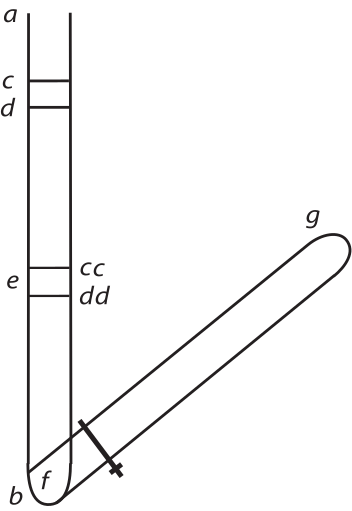
\includegraphics[width=0.4\textwidth]{images/37_3_111r}
                        %\caption{Bildbeschreibung}
                    %    \end{wrapfigure}
                        %@ @ @ Dies ist eine Abstandszeile - fuer den Fall, dass mehrere figures hintereinander kommen, ohne dass dazwischen laengerer Text steht. Dies kann zu einer Fahlermeldung fuehren. @ @ @ \\
                     \edtext{seu}{\lemma{$\displaystyle1\protect\frac{1}{2}$.}\Afootnote{ \textit{ (1) }\ Ergo ut sit aequalitas \textit{ (2) }\ seu \textit{ L}}} corpora 4. spatia 3. distributa ergo aequaliter compressione\protect\index{Sachverzeichnis}{compressio} semper quatuor partes aeris occupabunt tres loci v. g. quatuor decimae partes aeris totius occupabunt tres decimas partes loci. Quaeritur an ob apertum Epistomium\protect\index{Sachverzeichnis}{epistomium} \edtext{in \textit{b}}{\lemma{Epistomium}\Afootnote{ \textit{ (1) }\ \textit{bg} in \textit{f} \textit{ (2) }\ in \textit{b} \textit{ L}}} Mercurius\protect\index{Sachverzeichnis}{mercurius} sit ultra descensurus \edtext{quod negatur, est enim eadem in toto quantitas compressionis quae ante seu resistitur}{\lemma{descensurus}\Afootnote{ \textit{ (1) }\ . Et negatur, est enim eadem in toto quantitas compressionis\protect\index{Sachverzeichnis}{compressio|textit} quam ante. Et demonstratio haec est, ponatur descendere longius \textit{ (2) }\ quod [...] resistitur \textit{ L}}} 
                     [111 v\textsuperscript{o}] ei ab eodem aere a quo ante resistebatur, etsi per spatium latius disperso. Ergo in caeterum novi spatii aerem nihil potest, cum vis ejus omnis jam a priore aere contraponderetur. Claudatur Epistomium\protect\index{Sachverzeichnis}{epistomium}, profundius descendet Mercurius\protect\index{Sachverzeichnis}{mercurius} quia \edtext{minus}{\lemma{minus}\Afootnote{\textit{ (1) } Mercurii\ \textit{streicht Hrsg.}\ \textit{ (2) } aeris \textit{L}}} aeris ei nunc resistit. Est enim \edtext{\textit{eb}}{\lemma{}\Afootnote{\textit{eb} \textit{ erg.} \textit{ L}}} aer residuus \edtext{sub}{\lemma{residuus}\Afootnote{ \textit{ (1) }\ e \textit{ (2) }\ in \textit{ (3) }\ sub \textit{ L}}} Mercurio\protect\index{Sachverzeichnis}{mercurius}\edtext{}{\lemma{}\Afootnote{Mercurio  \textbar\ \textit{eb} \textit{ erg. u.}\  \textit{ gestr.}\ \textbar\ non \textit{ L}}} non \edtext{amplius aequalis aeri \textit{fg}}{\lemma{amplius}\Afootnote{ \textit{ (1) }\ dimidium aeris \textit{efg} vel quod idem (posito \textit{db} et \textit{fg} esse aeque longum \textit{ (2) }\ aequalis aeri \textit{fg} \textit{ L}}} ut erat initio cum Epistomium\protect\index{Sachverzeichnis}{epistomium} primum aperiretur, sed erit pars ejus dimidia \edtext{seu}{\lemma{dimidia}\Afootnote{ \textit{ (1) }\ jam eadem vis quae potest \textit{ (2) }\ seu \textit{ L}}} pars tertia totius aeris qui implevit \textit{db-fg} cum antea fuerit pars dimidia. Erit ergo pars una et dimidia aeris comprehendentis spatium duplum. Ecce ergo spatium dimidiatum, at corpus non duplicatum. Spatia sunt ut 2. ad 1. corpora ut 1 ad $\rule[-4mm]{0mm}{10mm}1\displaystyle\frac{1}{2}$. Jam quicquid comprimere potest corpus ut 1. ad spatium \edtext{dimidium prioris}{\lemma{dimidium}\Afootnote{prioris \textit{ gestr. und wieder g\"ultig gemacht} \textit{ L}}}, id comprimere poterit corpus $\rule[-4mm]{0mm}{10mm}1\displaystyle\frac{1}{2}$ in spatium quod sit ad prius ut est 1 ad $\rule[-4mm]{0mm}{10mm}1\displaystyle\frac{1}{2}$ descendet ergo \mercury\ per quartam partem spatii \textit{eb} sed aperto Epistomio\protect\index{Sachverzeichnis}{epistomium} rursus ascendet, idque continua reciprocatione, quae mira videbitur intuenti, nec ratio facile a quovis divinabitur. Quanto autem major est Tubus alter [\textit{gf}]\edtext{}{\lemma{\textit{bf}}\Afootnote{\textit{\ L \"{a}ndert Hrsg.}}}  tanto plus clauso rursus Epistomio\protect\index{Sachverzeichnis}{epistomium} descendet Mercurius\protect\index{Sachverzeichnis}{mercurius}, et si Tubus %\edtext{}{\Afootnote{\textit{bf}\textit{\ L \"{a}ndert Hrsg. } }}
\edtext{[\textit{gf}]}{\lemma{\textit{bf}}\Afootnote{\textit{\ L \"{a}ndert Hrsg.}}}\edtext{ maximus ad altitudinem usque atmosphaerae}{\lemma{[\textit{gf}]}\Afootnote{ \textit{ (1) }\ sit maximus, tota scilicet Atmosphaera\protect\index{Sachverzeichnis}{atmosphaera|textit} seu aer liber clauso al \textit{ (2) }\ maximus ad altitudinem usque atmosphaerae \textit{ L}}} assurgens fingatur, tantundem ad sensum descendet Mercurius\protect\index{Sachverzeichnis}{mercurius} vice secunda quantum prima, modo scilicet pondus\protect\index{Sachverzeichnis}{pondus} ejus alioquin ponderi atmosphaerae \edtext{praevaleat,}{\lemma{atmosphaerae}\Afootnote{ \textit{ (1) }\ praeponderet. \textit{ (2) }\ praevaleat, \textit{ L}}} seu modo sit numero pollicum praescripto major.
\pend